\documentclass{FR16} 

\begin{document}

\maketitle

% ML template reports
% https://www.cs.utexas.edu/~mooney/cs391L/paper-template.html
%https://github.com/udacity/machine-learning/blob/master/projects/capstone/report-example-1.pdf
\newpage
\tableofcontents
\newpage
\section{Abstract}
The aim of the project is to analyse and develop prediction models for the data from the "New York City Airbnb Open Data" from a Kaggle competition.
\\ In particular, one part is focused on the developing predictive model to forecast house prices using Supervised Learning technics:\begin{itemize}
\itemsep0em 
\item Linear Regression
\item Decision Tree
\item Random Forest
\item Ranger Random Forest
\item Neural Newtworks (?)
\end{itemize}
The second part is focused on the clusterisation of the data using Unsupervised Learning technics: Cluster Analysis and K-means algorithm.
\begin{itemize}
\itemsep0em
\item Cluster Analysis
\item K-means Algorithm
\end{itemize}
A crucial part of the project was to the tuning and finding of the hyperparameters of the different models in order to get the best fit.
%%Eachreport must contain:\\
%•shortabstract: what are your going to present %in the report\\
%•statementof the problem/goalof the analysis %and description of thedata set(s)\\
%•list of three to fivefindings/keypoints\\
%•the analysis with wisecommentary\\
%•(optional) theoretical background of the used %methods\\
%•conclusions(should include the findings/%keypoints)\\
%•theAppendix, containing all the R codeNotice:
%\\•Thepaper lengthisirrelevant provided that %the content is correct.
%\\•No R code in the main text.The R code must %be confined to the appendix\\
%•The report should be prepared inPDFonly

\newpage
\section{Problem Definition and Algorithm}
\subsection{Two main Goal}
\textbf{Develope predicting models for price}\\
The project is focused on a AirBnB user point of view. It is possible to image an application in which the user has a lot of information depending on the objective. For a landlord point of view, giving the information about the longitude and the latitude of the house, he/she will have as output the estimated price given based also on the neighbourhood group in New York City. For a guest point of view, he/she will give in input information about the price range and the type of room to get as output the most suitable houses for him or predict the position of one of that.\\\\
\textbf{Define clusters and groups}\\
For the Unsupervised part, the goal is to define cluster of price in which is possible to split out the houses, firstly in the entire city, secondly filtering for Neighborhood or room type. 

\#\# FOR A SPECIFIC NEIGHBOORHOOD OR FOR THE ENTIRE NY CITY
\subsection{Algorithms}
\subsubsection{Linear Regression}
 Linear regression  is a linear approach to modeling the relationship between a dependent variable and one or more independent variables. Linear regression should be suitable, since there could be a linear relationship between the position and the price. In the city center there will be the expensive houses, while in the outskirts there will be the cheaper ones.
  \subsubsection{Decison Trees}
In decision analysis, a decision tree can be used to visually and explicitly represent decisions and decision making.

 \subsubsection{Random Forest}
 Random forests are an ensemble learning method for classification, regression and other tasks that operate by constructing a multitude of decision trees.
 \subsubsection{Ranger Random Forest}
Ranger is a fast implementation of random forests or recursive partitioning, particularly suited for high dimensional data. 

 
\newpage
\section{Experimental Evaluation}

\subsection{Methodology}
\subsubsection{Data Inspection}
The dataset used in this project is one of a Kaggle competiotion and is called the New York City Airbnb Open Data. It contains 48.000 data points for each different column.
The dataset has different columns: 
\begin{itemize}
\itemsep0em 
\item id
\item \textbf{name}: name of the listing
\item \textbf{host\_id}
\item \textbf{host\_name}
\item \textbf{neighbourhood\_group}: location
\item \textbf{neighbourhood}: area
\item \textbf{latitude}: coordinates
\item \textbf{longitude}: coordinates
\item \textbf{room\_type}: space type
\item \textbf{price}:  in dollars
\item \textbf{minimum\_nights}: amount of nights minimum
\item \textbf{number\_of\_reviews}: number of reviews
\item \textbf{last\_review}: latest review
\item \textbf{reviews\_per\_month}: number of reviews per month
\item \textbf{calculated\_host\_listings\_count}: amount of listing per host
\item  \textbf{availability\_365}: number of days when listing is available for booking\\
\end{itemize}
We select just 5 of this feature from the dataset since we denotes them as the most important for the price of a house: latitude, longitude, room type, neighbourhood and the price itself to compare the prediction during the tests. \\\\
From the Figure 1 is possible to see that there are some outliers in the dataset that could be removed, but only by a choise of the user, since it is possible that someone wants to rent a luxury house. In fact, no outlier was removed from the dataset. Also, there were no null and missing value apart from the reviews\_per\_month column that we do not take in account in the project.
\\
\\From Figure2, it is possible to see the distribution of all houses in New York City and the price. Moreover, it can be noticed that the prices for the most part are in the range $0$-$500\$$ and only some istances have a price greater than $1000\$$. Also, the fact that some houses have a cost of $0\$$ is strange, nobody rent a house for free.
 \begin{figure}[H]
\centering
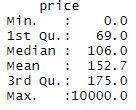
\includegraphics[width=0.3\textwidth]{figures/figure1.jpg} 
\caption{\label{fig:1}Price summary}
\end{figure}
\begin{figure}[H]
\centering
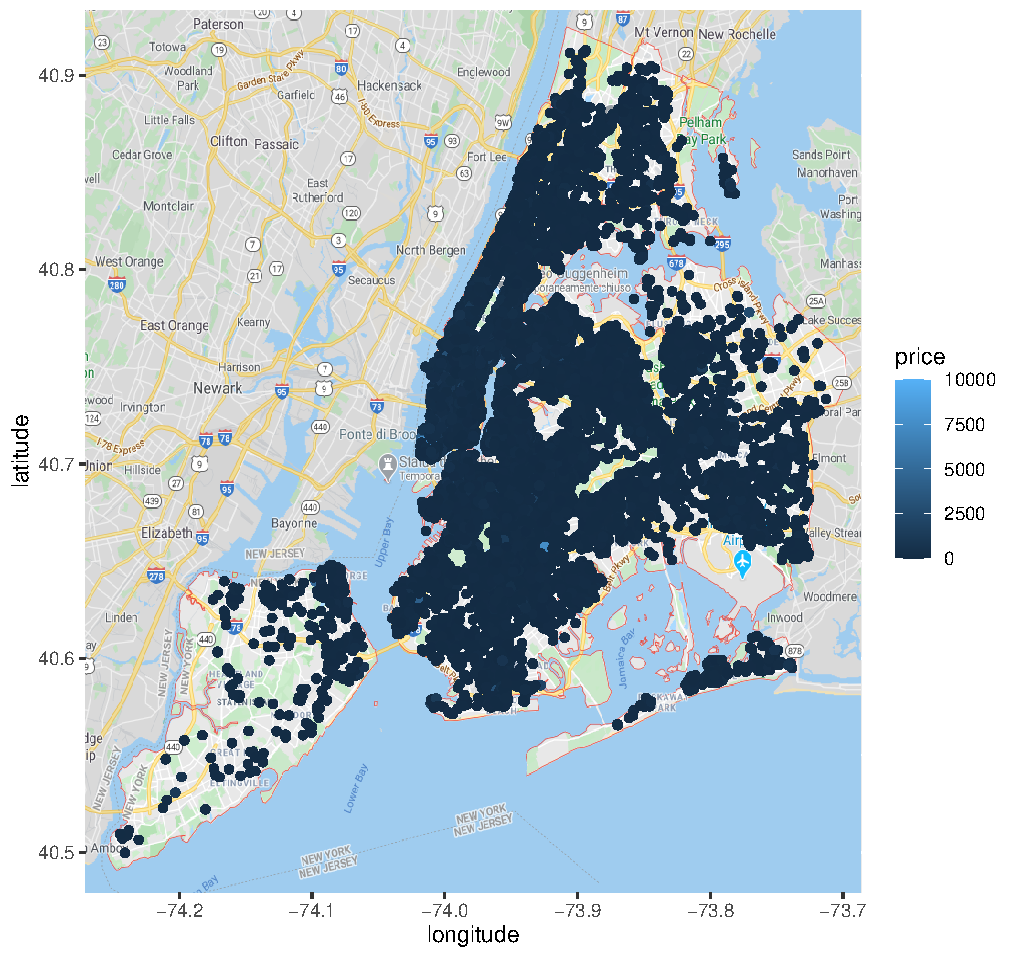
\includegraphics[width=0.5\textwidth]{figures/figure2.pdf} 
\caption{\label{fig:2}Distribution of all houses in NY colored by prices}
\end{figure}

\subsubsection{Data Cleaning and Pre-processing}
The dataset has more or less 48.000 data points for each column, so an important part of this work was the pre-processing since the large amount of data. Moreover, running different methods and algorithms on the entire dataset has an high computation cost. An important choice to made is that the user is able to discriminate which type of house has a particular interest. Then, it can be assume that the user chooses which is the price range of interest and also the type of room. For the simplicity of the project we will focus on the Manhattan region for the popularity, a range of price from $15\$$ to $500\$$ and an entire apartment type of room. The project can be extended easily to the entire dataset, based on the user preference. 
Each variable choosed in this project have been rescaled to let the model perform and learn better, apart from latitude and longitude since the rescaling should not have a real meaning.
\\ Also categorical variables have been rescaled assigning a numerical value to each category, resulting as factors. \\
The selected categorical features are: neighbourhood\_group and room type.\\
The selected numerical features are: latitude, longitude and price.
\begin{figure}[H]
\centering
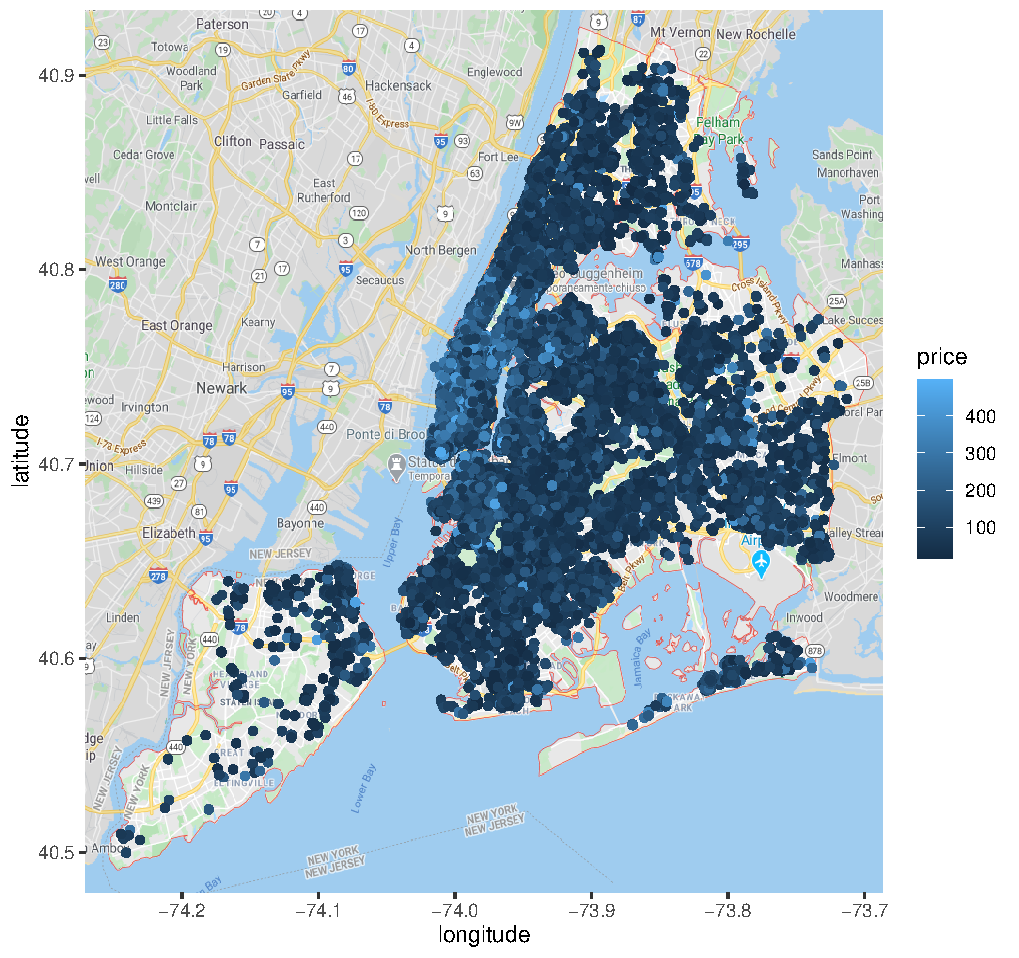
\includegraphics[width=0.5\textwidth]{figures/figure3.pdf} 
\caption{\label{fig:3} Distribution of all houses in NY of price between $15\$$ and $500\$$ per day}
\end{figure}

\begin{figure}[H]
\centering
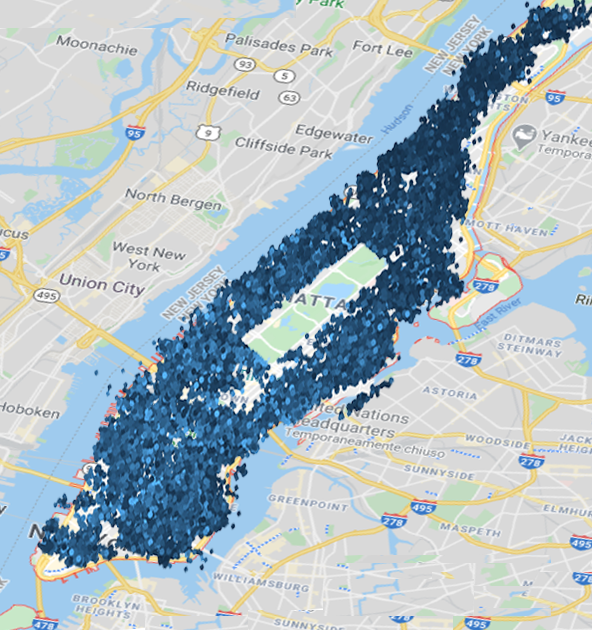
\includegraphics[width=0.5\textwidth]{figures/figure4.PNG} 
\caption{\label{fig:4}  Approximated distribution map of all houses in Manhattan }
\end{figure}



\subsection{Results}

\subsubsection{Linear Regression}
For the Linear regression the model give different results based on the variables used. \\\\
\textbf{Linear Regression selecting the Neighboorhood group}\\
For semplicity, the tests have been only taken filtering for Manhattan data points, but changing the neighboorhood the results are similar. 
Results are acceptable (Figure 5), given a $R^2$ value of $0.4011$ and a Mean Square Error, comparing prediction and test set, of $0.67$.
\\\\ \textbf{Linear Regression selecting the Neighboorhood group and the type of room}\\
As in the previous case the tests are for Manhattan and for Entire home/Aparment type of room.\\
The model output (Figure 6) a value of $R^2$ equals to $ 0.05953$ which is low  and a Mean Square Error, comparing prediction and test, of $1.23$.
\\\\ \textbf{Linear Regression without filters}\\
The model (Figure 7) obtain a $R^2$ value of $0.4031$ which is acceptable and a Mean Square Error, comparing prediction and test set, of $ 0.59$.
\begin{figure}[H]
\centering
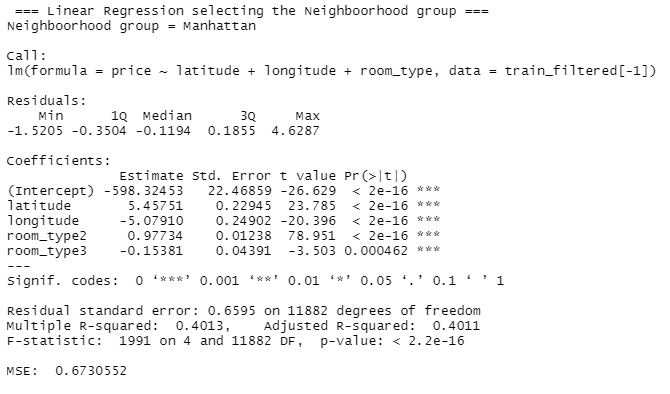
\includegraphics[width=0.5\textwidth]{figures/lm2.PNG} 
\caption{\label{fig:6}  Linear Regression output filtering by  Manhattan}
\end{figure}
\begin{figure}[H]
\centering
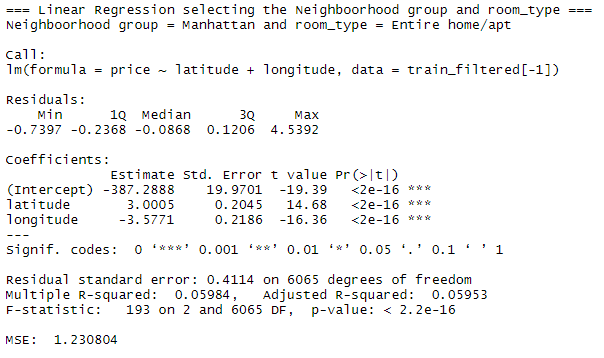
\includegraphics[width=0.5\textwidth]{figures/lm3.PNG} 
\caption{\label{fig:7}  Linear Regression output filtering by  Manhattan and Entire home/Apartment }
\end{figure}
\begin{figure}[H]
\centering
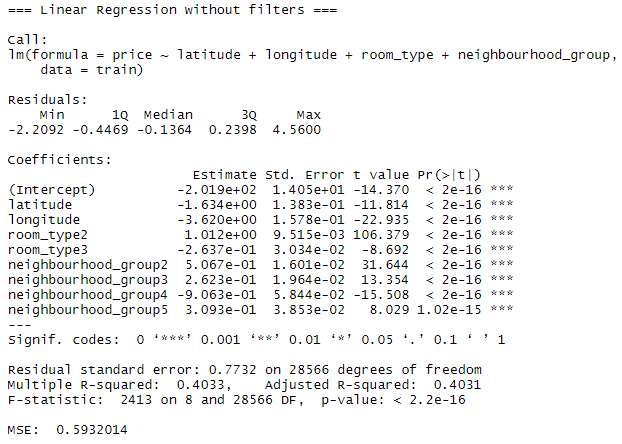
\includegraphics[width=0.5\textwidth]{figures/lm1.PNG} 
\caption{\label{fig:5} Linear Regression output without filters }
\end{figure}
\subsubsection{Decison Trees}

\subsubsection{Random Forest}

\subsubsection{Ranger Random Forest}


\subsection{Discussion}

\section{Conclusion}




\subsection{Decision Tree}
Decision  tree are one of the most used model in the Machine Learning world since are very familiar to human users and can be easily plotted. 
\\



\subsection{Random Forest}
Random Forest is an ensemble method which use a combination of decision tree to get the prediction.
\subsubsection{Ranger Random Forest}
Ranger Random Forest is a computationally light model which results are very close the classical Random Forest.
\\

\subsection{Linear Regression}



\newpage
\section{Results}
\subsection{Decision Tree}
\subsection{Random Forest results}
\subsection{Ranger Random Forest results}
\subsection{Linear Regression results}
\subsection{Neural Networks results}
\newpage
\section{Conclusion}
From the result the method with the most higher accuracy is the Random Forest method... while the worst are ....
\\Moreover, Random Forest method is also the worst in term of computation time for the tuning part since it takes for a configuration with 4 core, more or less 1 hour to tune the parameters. 


\newpage
\section{Appendix}

\newpage

\section{Tabelle e grafici}
Here a few examples of tables and graphs.
\subsection{Tabelle}
\begin{center}
\begin{tabular}{c c c c c c c c}
\arrayrulecolor{Azzurro}
\hline
{\bfseries $Codice$} & {\bfseries $CdL$} & {\bfseries $Lotto$} & {\bfseries $T_{setup/lotto}$} & {\bfseries $T_{lav/pezzo}$} & {\bfseries $T_{proc/pezzo}$} & {\bfseries$Quantit\grave{a}$} & {\bfseries $T_{tot}$}\\
\hline
100 & 4 & 250 & 25 & 0,5 & 0,6 & 1 & 0,6\\
111 & 2 & 250 & 20 & 2 & 2,08 & 1 & 2,08 \\
111 & 3 & 250 & 15 & 1,5 & 1,56 & 1 & 1,56 \\
112 & 2 & 250 & 20 & 2,5 & 2,58 & 1 & 2,58 \\
112 & 3 & 250 & 15 & 2 & 2,06 & 1 & 2,06\\
113 & 3 & 500 & 15 & 1 & 1,03 & 2 & 2,06\\
120 & 1 & 50 & 30 & 2 & 2,6 & 0,1 & 0,26\\
121 & 1 & 25 & 30 & 3 & 4,2 & 0,1 & 0,42 \\
121 & 1 & 25 & 30 & 2,5 & 3,7 & 0,1 & 0,37 \\
\hline
\end{tabular}
\end{center}

\subsubsection{Altra tabella}
\subsection{Grafici}
\begin{center}

\end{center}



\section{Altro}
\begin{figure}[H]
\centering
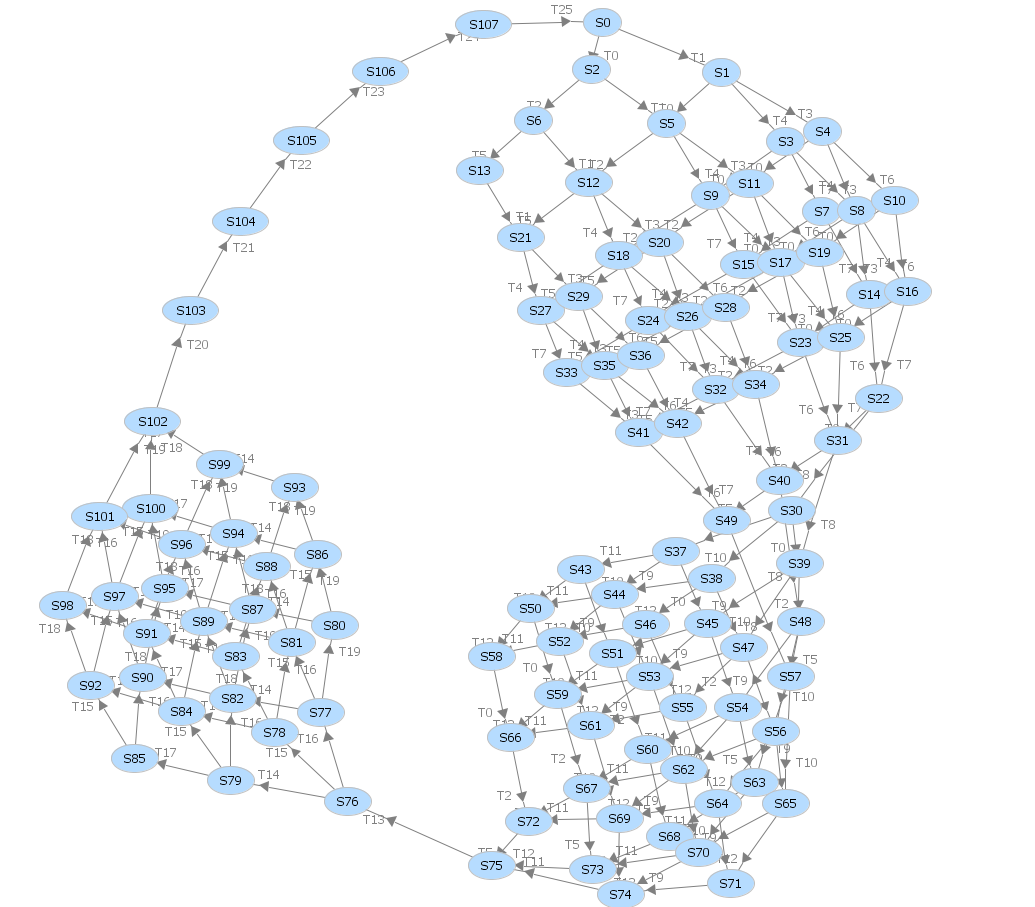
\includegraphics[width=1\textwidth]{grafo.png}
\caption{\label{fig:1}Didascalia.}
\end{figure}
\subsection{Footnote}
You can create a footnote like this.\footnote{I created a footnote.}



\newpage
\begin{thebibliography}{9}
\bibitem{giusti}
Giusti, Santochi, \emph{Tecnologia Meccanica e Studi di Fabbricazione}. Casa Editrice Ambrosiana, Seconda Edizione
\bibitem{mechteacher}
Mechteacher, \emph{Knuckle Joint – Introduction, Parts and Applications},\\ http://mechteacher.com/knuckle-joint/
\bibitem{totalmateria}
Totalmateria, \emph{G32NiCrMo8}, http://www.totalmateria.com 
\bibitem{sandvik}
Sandvik Coromant,\emph{Catalogo  generale  2018},   http://www.coromant.sandvik.com/it
\bibitem{uni}
Norme UNI, Ente nazionale italiano di unificazione
\end{thebibliography}

\end{document}